% Options for packages loaded elsewhere
\PassOptionsToPackage{unicode}{hyperref}
\PassOptionsToPackage{hyphens}{url}
%
\documentclass[
]{article}
\usepackage{amsmath,amssymb}
\usepackage{lmodern}
\usepackage{ifxetex,ifluatex}
\ifnum 0\ifxetex 1\fi\ifluatex 1\fi=0 % if pdftex
  \usepackage[T1]{fontenc}
  \usepackage[utf8]{inputenc}
  \usepackage{textcomp} % provide euro and other symbols
\else % if luatex or xetex
  \usepackage{unicode-math}
  \defaultfontfeatures{Scale=MatchLowercase}
  \defaultfontfeatures[\rmfamily]{Ligatures=TeX,Scale=1}
\fi
% Use upquote if available, for straight quotes in verbatim environments
\IfFileExists{upquote.sty}{\usepackage{upquote}}{}
\IfFileExists{microtype.sty}{% use microtype if available
  \usepackage[]{microtype}
  \UseMicrotypeSet[protrusion]{basicmath} % disable protrusion for tt fonts
}{}
\makeatletter
\@ifundefined{KOMAClassName}{% if non-KOMA class
  \IfFileExists{parskip.sty}{%
    \usepackage{parskip}
  }{% else
    \setlength{\parindent}{0pt}
    \setlength{\parskip}{6pt plus 2pt minus 1pt}}
}{% if KOMA class
  \KOMAoptions{parskip=half}}
\makeatother
\usepackage{xcolor}
\IfFileExists{xurl.sty}{\usepackage{xurl}}{} % add URL line breaks if available
\IfFileExists{bookmark.sty}{\usepackage{bookmark}}{\usepackage{hyperref}}
\hypersetup{
  pdftitle={Variation in myoglobin content of skeletal muscle of seal species.},
  pdfauthor={Emma Rand},
  hidelinks,
  pdfcreator={LaTeX via pandoc}}
\urlstyle{same} % disable monospaced font for URLs
\usepackage[margin=1in]{geometry}
\usepackage{longtable,booktabs,array}
\usepackage{calc} % for calculating minipage widths
% Correct order of tables after \paragraph or \subparagraph
\usepackage{etoolbox}
\makeatletter
\patchcmd\longtable{\par}{\if@noskipsec\mbox{}\fi\par}{}{}
\makeatother
% Allow footnotes in longtable head/foot
\IfFileExists{footnotehyper.sty}{\usepackage{footnotehyper}}{\usepackage{footnote}}
\makesavenoteenv{longtable}
\usepackage{graphicx}
\makeatletter
\def\maxwidth{\ifdim\Gin@nat@width>\linewidth\linewidth\else\Gin@nat@width\fi}
\def\maxheight{\ifdim\Gin@nat@height>\textheight\textheight\else\Gin@nat@height\fi}
\makeatother
% Scale images if necessary, so that they will not overflow the page
% margins by default, and it is still possible to overwrite the defaults
% using explicit options in \includegraphics[width, height, ...]{}
\setkeys{Gin}{width=\maxwidth,height=\maxheight,keepaspectratio}
% Set default figure placement to htbp
\makeatletter
\def\fps@figure{htbp}
\makeatother
\setlength{\emergencystretch}{3em} % prevent overfull lines
\providecommand{\tightlist}{%
  \setlength{\itemsep}{0pt}\setlength{\parskip}{0pt}}
\setcounter{secnumdepth}{5}
\ifluatex
  \usepackage{selnolig}  % disable illegal ligatures
\fi
\newlength{\cslhangindent}
\setlength{\cslhangindent}{1.5em}
\newlength{\csllabelwidth}
\setlength{\csllabelwidth}{3em}
\newenvironment{CSLReferences}[2] % #1 hanging-ident, #2 entry spacing
 {% don't indent paragraphs
  \setlength{\parindent}{0pt}
  % turn on hanging indent if param 1 is 1
  \ifodd #1 \everypar{\setlength{\hangindent}{\cslhangindent}}\ignorespaces\fi
  % set entry spacing
  \ifnum #2 > 0
  \setlength{\parskip}{#2\baselineskip}
  \fi
 }%
 {}
\usepackage{calc}
\newcommand{\CSLBlock}[1]{#1\hfill\break}
\newcommand{\CSLLeftMargin}[1]{\parbox[t]{\csllabelwidth}{#1}}
\newcommand{\CSLRightInline}[1]{\parbox[t]{\linewidth - \csllabelwidth}{#1}\break}
\newcommand{\CSLIndent}[1]{\hspace{\cslhangindent}#1}

\title{Variation in myoglobin content of skeletal muscle of seal species.}
\author{Emma Rand}
\date{}

\begin{document}
\maketitle

{
\setcounter{tocdepth}{2}
\tableofcontents
}
\hypertarget{introduction}{%
\section{Introduction}\label{introduction}}

Aquatic and marine mammals are able to dive underwater for extended periods as a result of having a higher muscle myoglobin concentration than terrestrial mammals (Kanatous and Mammen 2010). (Allaire et al. 2019) found that 83\% of the variation in Toothed whale species (odontocetes) dive capacity was accounted for by body mass and myoglobin content.
Seal species are also known to vary in dive length. We investigated whether the concentration of myoglobin differed between three species of seal: Weddell Seal, Harbour Seals and Bladdernose Seals. See Figure \ref{fig:weddell-fig}



\begin{figure}
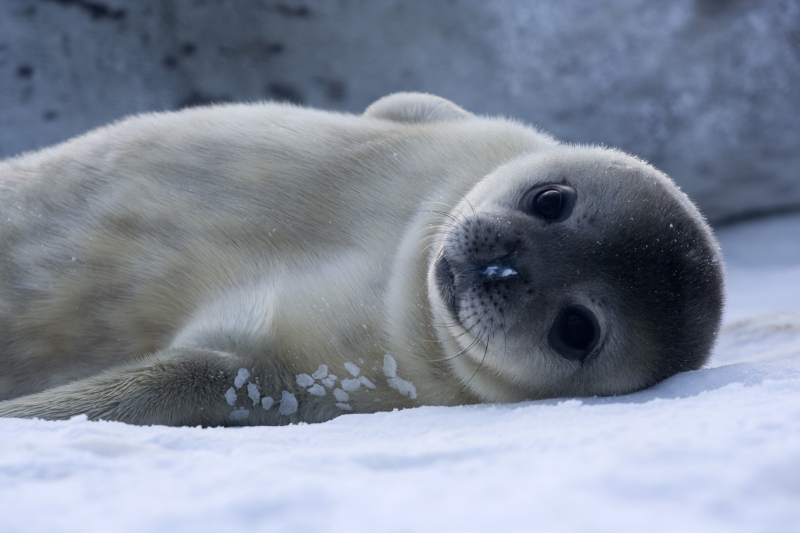
\includegraphics[width=3.7in,height=200px]{pics/Baby_Weddell_Seal} \caption{Baby Weddell Seals are very cute. By Photo © Samuel Blanc, CC BY-SA 3.0, \url{https://commons.wikimedia.org/w/index.php?curid=3877642}}\label{fig:weddell-fig}
\end{figure}

\hypertarget{methods}{%
\section{Methods}\label{methods}}

We measured the myoglobin content of the skeletal muscle of 28 individuals in each of three species.
We used R (R Core Team 2019) with tidyverse packages (Wickham 2017) for all analyses and the rmarkdown (Allaire et al. 2019) and bookdown (Xie 2016) packages for manuscript preparation.

\hypertarget{results}{%
\section{Results}\label{results}}

There is a significant difference in myoglobin concentration between species (\emph{F} = 5.88; \emph{d.f.} =2, 81; \emph{p} = 0.004). Post-hoc testing revealed that difference to be between the Weddell seal with the highest myoglobin concentrations (\(\bar{x} \pm s.e.\): 48.91 \(\pm\) 1.61 g Kg\textsuperscript{-1}) and the Harbour seal with the lowest (41.6 \(\pm\) 1.46 g Kg\textsuperscript{-1}). See Figure \ref{fig:myo-fig}.
I've also gratuitously included a table with the same information just for the sake of including a table. See Table \ref{tab:summary-table}.

\begin{table}

\caption{\label{tab:summary-table}A summary of the data.}
\centering
\begin{tabular}[t]{l|r|r|r|r}
\hline
species & mean & std & n & se\\
\hline
Bladdernose & 44.44 & 7.82 & 28 & 1.48\\
\hline
Harbour & 41.60 & 7.75 & 28 & 1.46\\
\hline
Weddell & 48.91 & 8.54 & 28 & 1.61\\
\hline
\end{tabular}
\end{table}



\begin{figure}
\includegraphics[width=288px]{paper_files/figure-latex/myo-fig-1} \caption{Mean Myoglobin content of skeletal muscle. Error bars are \(\pm 1 s.e.\)}\label{fig:myo-fig}
\end{figure}

\hypertarget{discussion}{%
\section{Discussion}\label{discussion}}

Here we pick up points from the introduction. See \ref{introduction}.

\hypertarget{references}{%
\section*{References}\label{references}}
\addcontentsline{toc}{section}{References}

\hypertarget{refs}{}
\begin{CSLReferences}{1}{0}
\leavevmode\hypertarget{ref-markdown1}{}%
Allaire, JJ, Yihui Xie, Jonathan McPherson, Javier Luraschi, Kevin Ushey, Aron Atkins, Hadley Wickham, Joe Cheng, Winston Chang, and Richard Iannone. 2019. \emph{Rmarkdown: Dynamic Documents for r}. \url{https://github.com/rstudio/rmarkdown}.

\leavevmode\hypertarget{ref-Kanatous2741}{}%
Kanatous, Shane B., and Pradeep P. A. Mammen. 2010. {``Regulation of Myoglobin Expression.''} \emph{Journal of Experimental Biology} 213 (16): 2741--47. \url{https://doi.org/10.1242/jeb.041442}.

\leavevmode\hypertarget{ref-R-core}{}%
R Core Team. 2019. \emph{R: A Language and Environment for Statistical Computing}. Vienna, Austria: R Foundation for Statistical Computing. \url{https://www.R-project.org/}.

\leavevmode\hypertarget{ref-tidyverse}{}%
Wickham, Hadley. 2017. \emph{Tidyverse: Easily Install and Load the 'Tidyverse'}. \url{https://CRAN.R-project.org/package=tidyverse}.

\leavevmode\hypertarget{ref-bookdown}{}%
Xie, Yihui. 2016. \emph{Bookdown: Authoring Books and Technical Documents with {R} Markdown}. Boca Raton, Florida: Chapman; Hall/CRC. \url{https://github.com/rstudio/bookdown}.

\end{CSLReferences}

\end{document}
